\section{Introduction}
\label{sec:intro}

Linear probes often recover a correct answer from a language model's hidden states when the
model's own output is wrong. This representation--output gap has been studied for factual and
character-level tasks \citep{kappa,early_encode,inside_out,hiraoka_inui}, and it is often read as
evidence that the model has the answer but fails to express it. For character properties that
reading skips a step. The last letter of a word is a fixed property of the word, and subword
embeddings are known to encode spelling \citep{kaushal2022tokens,itzhak2022spelling}. A probe at the
answer position may therefore read a property that was stored with the word, one that the
question caused the model to assemble, or both.

\begin{figure}[t]
  \centering
  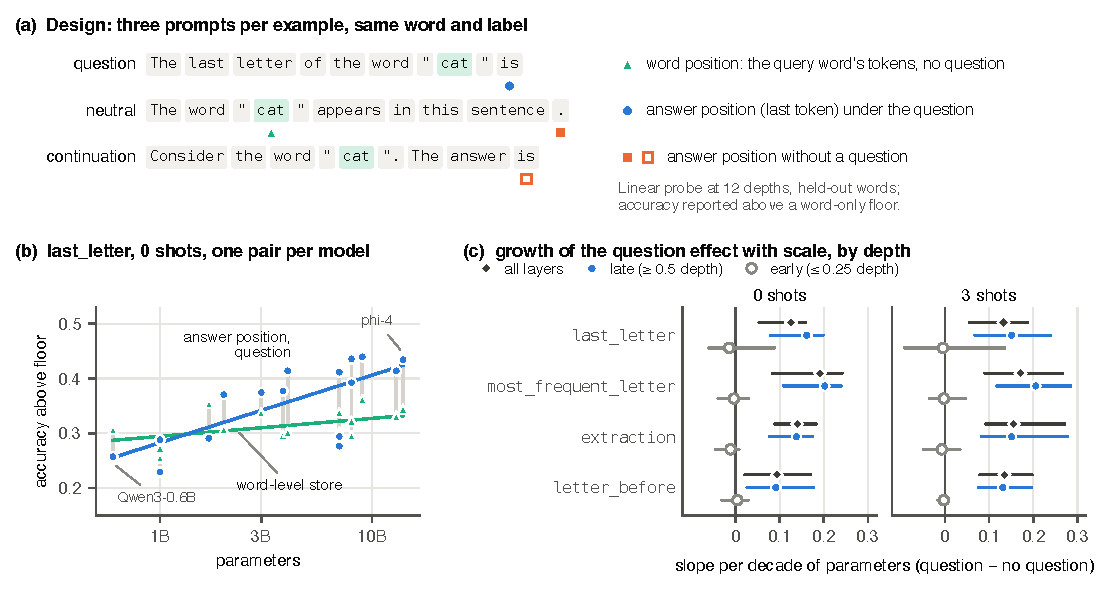
\includegraphics[width=\linewidth]{fig_overview.pdf}
  \caption{Overview: \texttt{last\_letter}, zero shots, one point per model, probe accuracy above
    the word-only floor. Right: two of the three prompts and the positions that a linear probe,
    trained and tested on disjoint words, reads. The store is read at the word's own tokens in the
    neutral sentence (held-out layer selection); answer-position points use the most accurate probed
    layer within the late ($\geq 0.5$) or early ($\leq 0.25$) depth band. Lines: OLS fits; grey
    segments join each model's late answer position under the question to its store. The store does
    not grow reliably with scale and the early signal is similar at every scale; the late signal under
    the question grows, and lies below the store in the smallest models and above it in the largest
    (\S\ref{sec:question}; Figure~\ref{fig:twophase}b).}
  \label{fig:overview}
\end{figure}

We separate these with a \emph{word-position baseline}: the same held-out-word probe, applied to
the query word's own tokens inside a sentence that asks nothing
(\texttt{The word "cat" appears in this sentence.}). Under causal attention those tokens have seen
only \texttt{The word "}, so their decodability is the closest available measure of what the model
stores about the word independently of any task. We compare it with the answer position under
the task question and under two question-free carriers, for 16 open-weight models from seven
families (0.6B--14B) and eleven character tasks, using held-out-word cross-validation, a word-only
nuisance floor, held-out layer selection, and pre-registered decision criteria.

Three results organize the paper.

\paragraph{A prompt-independent store exists, and it is mostly lexical.}
The word tokens encode \texttt{first\_letter}, \texttt{last\_letter} and
\texttt{most\_frequent\_letter} above the nuisance floor in all 16 models
(\S\ref{sec:store}). Roughly 70\% of that above-floor signal is already present at layer 0, in the
token embedding, consistent with prior work on spelling in embeddings. This half of the picture is
confirmation, not discovery, but it supplies the baseline that the rest of the analysis needs.

\paragraph{Asking adds a late signal, and only that signal grows with scale.}
At the answer position, the difference between the question prompt and the question-free carrier
grows with log parameter count for all four prompt-sensitive tasks, after Holm correction and
within model families (\S\ref{sec:question}; Figure~\ref{fig:twophase}b). Restricting the probe to layers past half depth
leaves the effect intact; restricting it to the first quarter removes it. The answer position of
small models holds less than their word-level store, while that of large models holds more
(Figure~\ref{fig:overview}). Layer
profiles show the two phases directly (Figure~\ref{fig:twophase}a): an early bump that is the same
at every scale, then a late rise that appears only in larger models.

\paragraph{Controls change what can be claimed.}
Measured against the word-only floor rather than the majority class, most of the question-free
signal that a majority-baseline analysis counts as retained is nuisance
(\S\ref{sec:question}). Count tasks fail the floor until length, letter repetition and query-letter
identity are removed by design (\S\ref{sec:nuisance}). Representation--readout gaps do not follow
a robust scaling trend once probe saturation is accounted for (\S\ref{sec:readout}). A
pre-registered stem-order experiment finds that placing the question before the word does not
change the word's encoding beyond what an arbitrary two-word prefix change does
(Appendix~\ref{app:prereg}).

\paragraph{Contributions.}
(1) A word-position baseline that separates prompt-independent storage from question-conditioned
decodability at the answer position. (2) Evidence that the scale-dependent part of character
decodability is late and question-driven, while early and word-level signals are scale-invariant.
(3) A set of controls (word-only floors with designed-out shortcuts, held-out layer selection,
pre-registration) that each reversed or removed a claim an uncontrolled analysis would have made.
We do not identify the mechanism behind the late signal; whether it reflects computation,
integration across the word's tokens, or reformatting is left open.
